
\chapter{Planning en taakverdeling}

% De initieel opgemaakte planning en de uiteindelijke uitvoering (in Ganttchart-achtige
% vorm) met een korte verklaring van de verschillen.

\subsubsection{Initiële planning}

Figuur \ref{fig:planning_initieel} op volgende pagina toont de initiële planning. De planning werd opgesteld naar aanleiding van de eerste presentatie en is bijgevolg relatief vaag en abstract. Desalniettemin is de initiële planning wel een rode lijn doorheen het volledige project gebleven. Naar aanleiding van de eerste presentatie is de toepassing namelijk grondig geanalyseerd en in kleinere subproblemen onderverdeeld.

In figuur \ref{fig:planning_initieel} wordt de gelaagde opbouw van Triump weergeven. De toepassing is namelijk ontwikkeld in 3 grote stappen of `cores'. Elke core vormt een mijlpaal in het ontwikkelproces en pas na uitvoerig testen wordt overgegaan naar de volgende core. 
Ten eerste is er de absolute basis van de applicatie zoals communicatie met de backend, het bepalen van de locatie van de gebruiker en een login en logout scherm. In de tweede core worden de basisonderdelen van Triump zoals locaties, events, rewards, groepen, gebruikers en een basis UI geïntegreerd in de applicatie. De laatste core richt zich voornamelijk op gebruiksvriendelijkheid en afwerking. In deze core bevinden zich elementen zoals een notificatiesysteem, instellingenpagina, feedbacksysteem en een aantrekkelijke UI.

Na het uitwerken van de kern werd tijd voorzien voor uitbreidingen. Mogelijke uitbreidingen waren: een iOS of WindowsPhone versie, integratie met bestaande diensten zoals Qustomer,... 

\subsubsection{Uiteindelijke planning en verschillen met initiële planning}

Figuur \ref{fig:planning_uiteindelijk} toont de uiteindelijke planning. In bovenstaande paragraaf werd de gelaagde opbouw van Triump reeds aangehaald. In deze planning werd elk onderdeel van deze lagen uitgewerkt teneinde een gedetailleerd overzicht te geven van de gevolgde werkwijze. Het grootste verschil met de initiële planning is de toevoeging van de webinterface. De nood aan een webinterface was gedurende de opstelling van de eerste planning niet gekend en werd pas gedurende de uitvoering van het project vastgesteld. Bijgevolg was het noodzakelijk de ontwikkeling van de webinterface te voorzien in de planning. 
Uit figuur \ref{fig:planning_uiteindelijk} volgt ook dat de initieel geplande uitbreidingen niet doorgevoerd zijn. Dit is voornamelijk te wijten aan de bijkomende taak, nl. de webinterface en de langere duurtijd van de tweede core.

\subsubsection{Taakverdeling}

Figuur \ref{fig:planning_uiteindelijk} geeft naast de planning ook de taakverdeling weer. De taken werden zo verdeeld dat de werklast evenredig opgesplitst werd over elk groepslid en dat iedereen zowel aan de frontend als aan de backend heeft gewerkt. Voor elk groepslid was het essentieel om in de verschillende onderdelen ervaring op te doen. Op deze manier heeft iedereen zowel over Androidontwikkeling, de backend, UI's,... een zekere kennis opgedaan. Voor kleinere taken zoals het oplossen van een bepaalde bug of het heropmaken van een UI element werd met `issues' gewerkt. Een `issue' is een beschrijving van een taak of een probleem en kan toegevoegd worden aan een git repository. Vervolgens kan een groepslid zich issues toeëigenen en proberen deze te verhelpen. Een voordeel van deze werkwijze is dat er een lijst opgesteld wordt van de openstaande en opgeloste problemen hetgeen efficiënt werken faciliteert.

\begin{figure}[H]
	\centering
	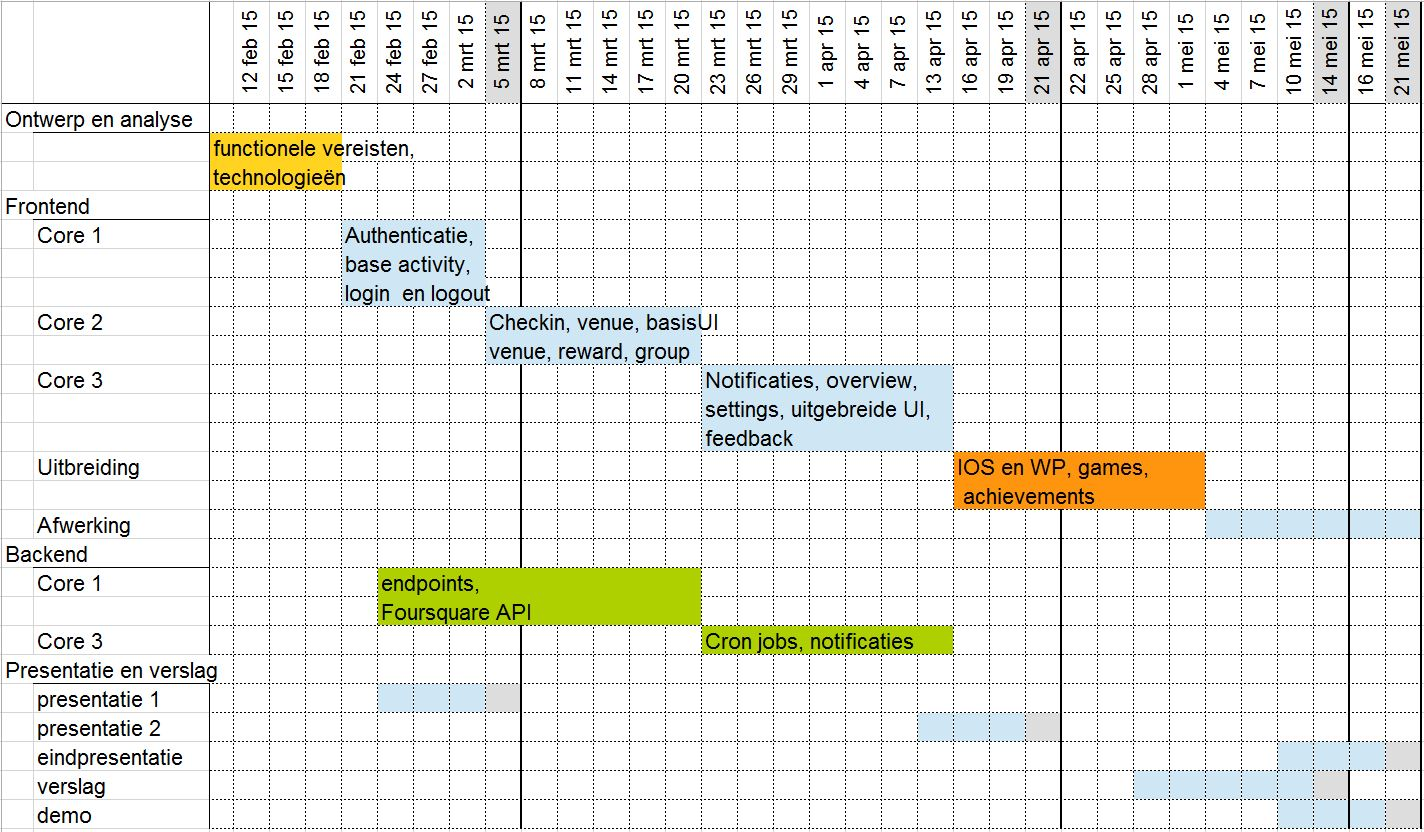
\includegraphics[scale=0.50, angle =90]{planning_initieel}
	\caption{Initieel opgemaakte planning}
	\label{fig:planning_initieel}
\end{figure}

\begin{figure}[H]
	\centering
	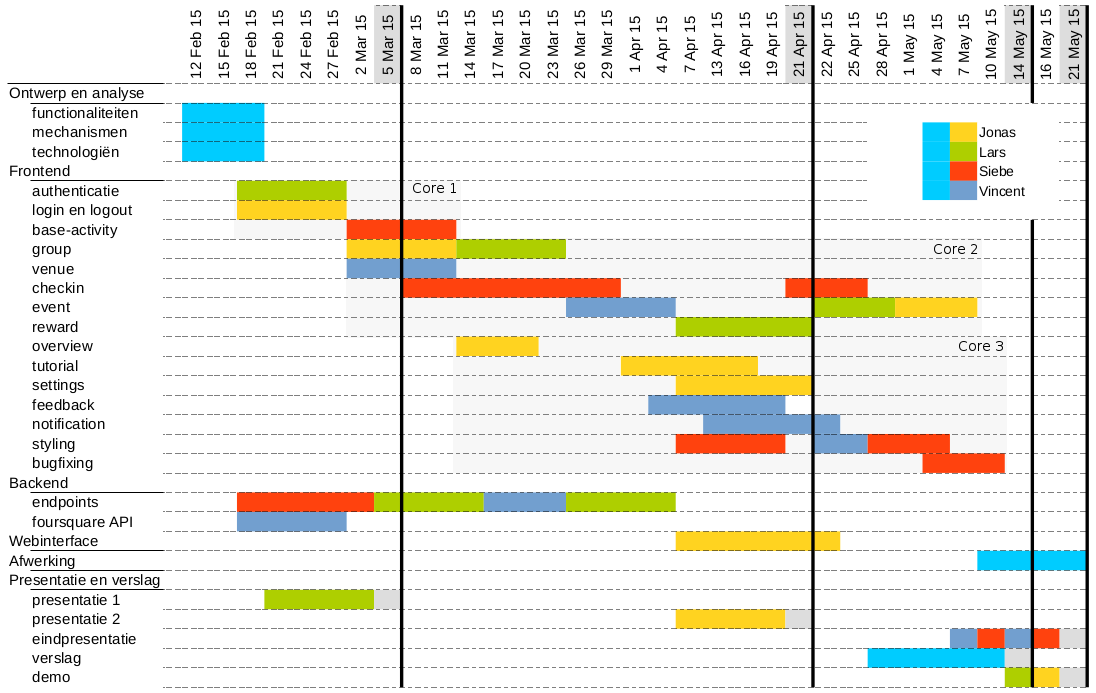
\includegraphics[scale=0.55, angle =90]{planning_2}
	\caption{Uiteindelijke planning}
	\label{fig:planning_uiteindelijk}
\end{figure}
